% ============================================================
% Figure Captions: Harmonic Molecular Resonator
% ============================================================

\begin{figure*}[!htbp]
    \centering
    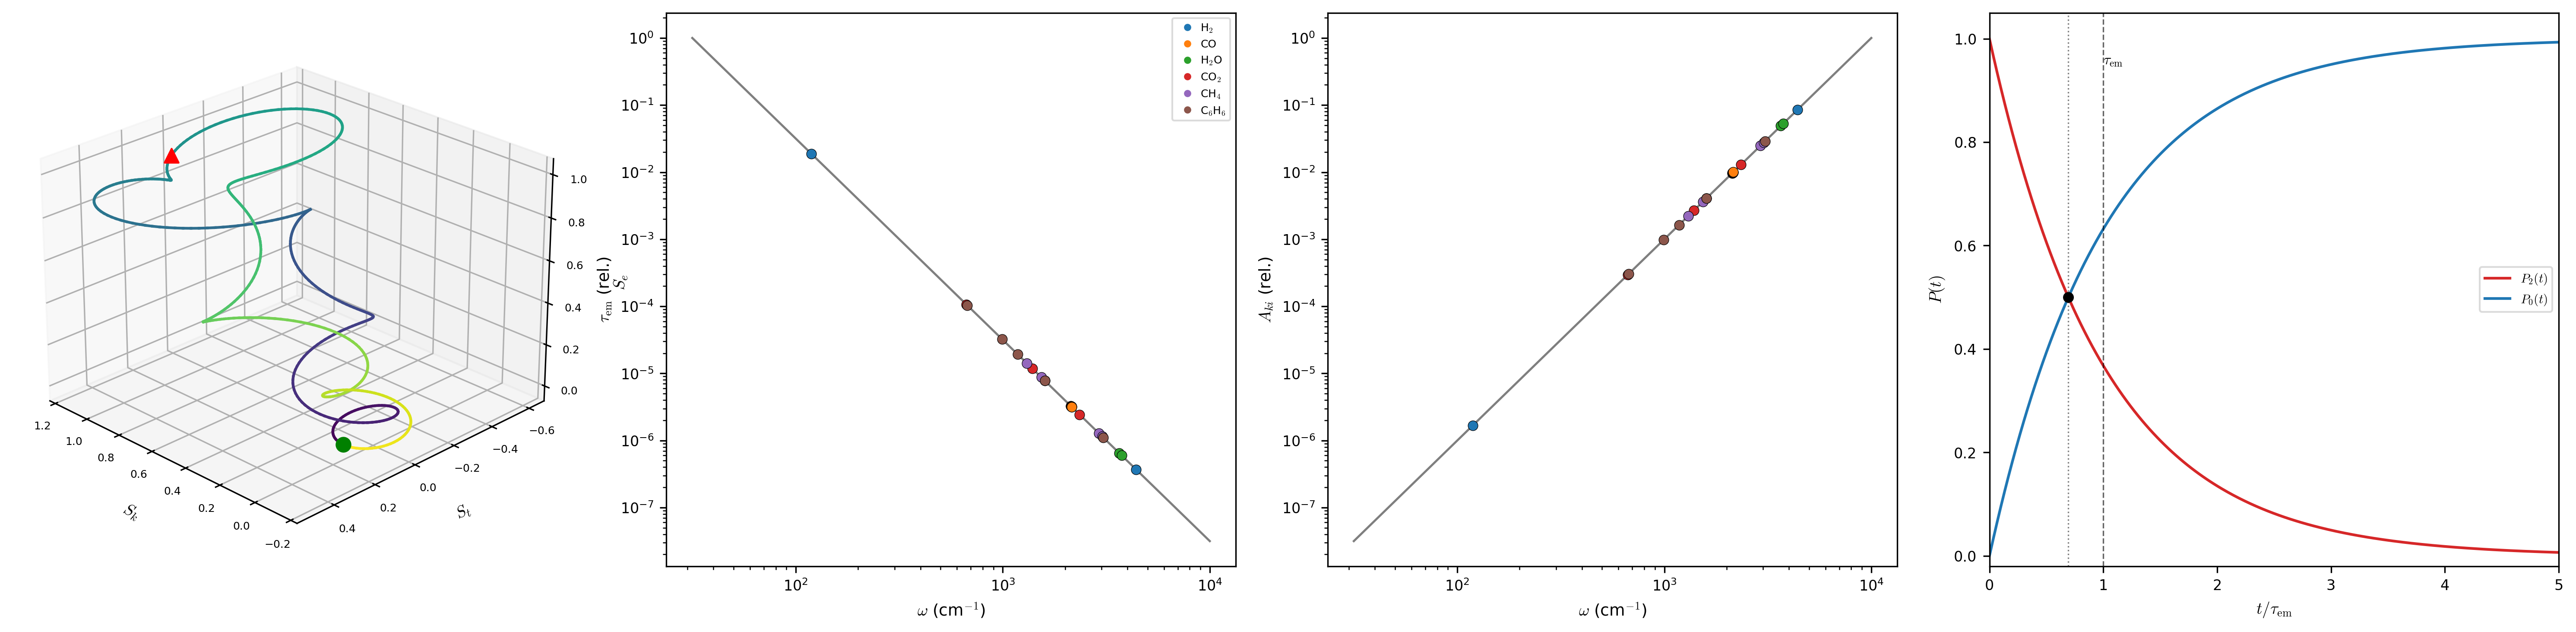
\includegraphics[width=\textwidth]{figures/panel_1_molecular_tick.png}
    \caption{\textbf{The Molecular Tick: Absorption-Emission as Categorical Cycle.}
    (\textbf{A})~Three-dimensional trajectory of a molecular absorption-emission cycle in S-entropy space $(\Sk, \St, \Se)$. The system begins at the ground state (bottom), spirals upward during photon absorption to the excited state (top torus), and decays back during spontaneous emission. The trajectory is coloured by time (yellow$\to$green$\to$blue), and the two circular orbits at ground and excited states represent the stationary categorical configurations. The emission lifetime $\tem$ marks one complete categorical cycle.
    (\textbf{B})~Emission lifetime versus vibrational frequency on logarithmic axes. The theoretical scaling $\tem \propto \omega^{-3}$ (dashed diagonal) follows from the Einstein A coefficient $A_{ki} = \omega_0^3 |\langle 0|\hat{\mu}|2\rangle|^2 / (3\pi\epsilon_0\hbar c^3)$. Points represent the fundamental modes of all six validation molecules, coloured by molecular type (diatomic$=$blue, triatomic$=$green, tetrahedral$=$orange, polyatomic$=$red). The spread about the theoretical line reflects variation in transition dipole moments.
    (\textbf{C})~Tick rate identity: categorical state transition rate $dM/dt = 1/\tem = A_{ki}$ versus frequency. The linear relationship on log-log axes confirms that the tick rate equals the Einstein A coefficient. Each point corresponds to one vibrational mode from the molecular database, with the diagonal reference line indicating exact proportionality.
    (\textbf{D})~Population dynamics during one emission cycle. Excited-state population $P_2(t) = e^{-t/\tem}$ (red, decaying) and ground-state population $P_0(t) = 1 - e^{-t/\tem}$ (blue, rising) versus normalised time $t/\tem$. The vertical dashed line at $t = \tem$ marks the emission lifetime---the point where the excited-state population has decayed to $1/e$. The crossing at $t = \tem \ln 2 \approx 0.69\,\tem$ marks equipartition between states. The interval $[0, \tem]$ constitutes one complete categorical tick.}
    \label{fig:molecular_tick}
\end{figure*}

\begin{figure*}[!htbp]
    \centering
    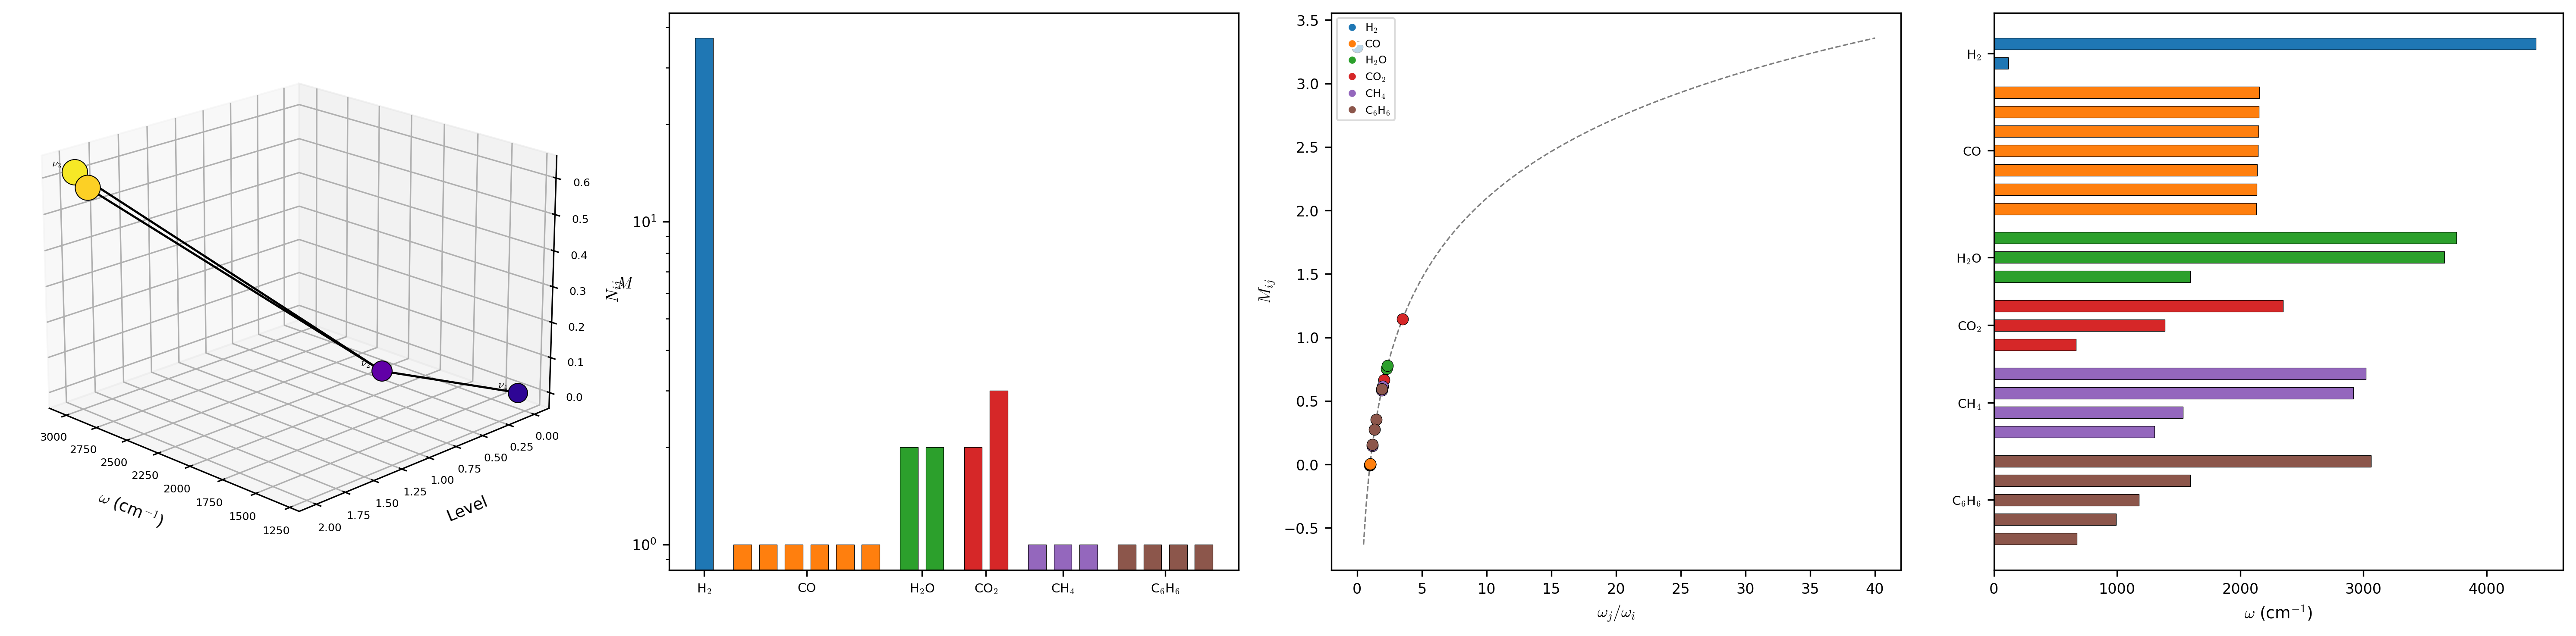
\includegraphics[width=\textwidth]{figures/panel_2_tick_hierarchy.png}
    \caption{\textbf{Nested Tick Hierarchy and Tree Structure.}
    (\textbf{A})~Three-dimensional tick tree for CH$_4$ (methane). Nodes represent vibrational modes plotted in (frequency, tree level, partition depth $\mathcal{M}$) space. The root node $\nu_4$ (1306~cm$^{-1}$) at level 0 connects downward to $\nu_2$ (1534~cm$^{-1}$) at level 1, which branches to $\nu_1$ (2917~cm$^{-1}$) and $\nu_3$ (3019~cm$^{-1}$) at level 2. Node size scales with subdivision number $N_{ij} = \lfloor\omega_j/\omega_i\rfloor$, and colour encodes frequency (blue$=$low, yellow$=$high). Solid lines are tree edges connecting parent to child.
    (\textbf{B})~Subdivision numbers $N_{ij}$ for all parent$\to$child tree edges across all six molecules. Each bar represents one edge, grouped and coloured by molecule. Most subdivision numbers are 1--3, reflecting the typical 2--3$\times$ frequency ratios between adjacent vibrational modes. The tall bar for H$_2$ ($N = 37$) reflects the large ratio between its vibrational and rotational frequencies.
    (\textbf{C})~Partition depth $\mathcal{M}_{ij} = \log_3(\omega_j/\omega_i)$ versus frequency ratio $\omega_j/\omega_i$ for all tree edges. The smooth $\log_3$ reference curve (solid line) passes through all data points, confirming that partition depth is the base-3 logarithm of the frequency ratio. Points are coloured by molecule. Higher frequency ratios produce deeper partition nesting.
    (\textbf{D})~Frequency ordering of all vibrational modes across the six molecules, displayed as horizontal bars sorted by frequency within each molecular group. Bar length is proportional to mode frequency in cm$^{-1}$, and colour identifies the molecule. This ordering defines the tree structure: within each molecule, the lowest-frequency mode is the tree root and higher-frequency modes are descendants. The frequency span from CCl$_4$ ($\nu_2 = 218$~cm$^{-1}$) to H$_2$ (4401~cm$^{-1}$) covers a factor of 20.}
    \label{fig:tick_hierarchy}
\end{figure*}

\begin{figure*}[!htbp]
    \centering
    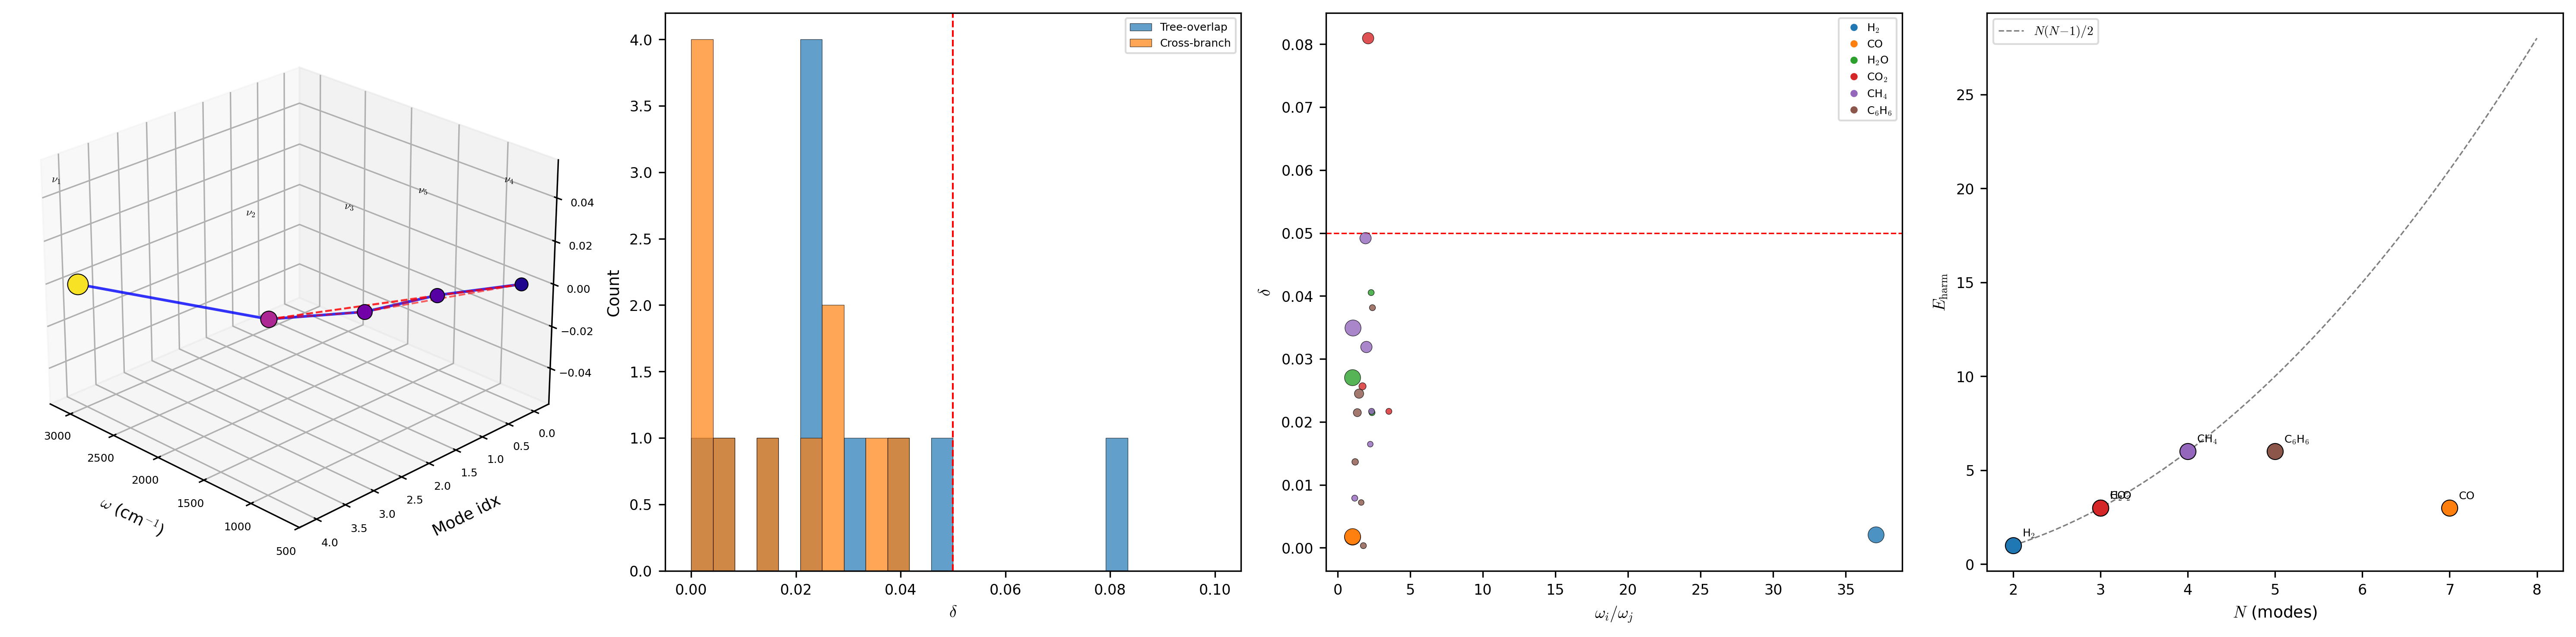
\includegraphics[width=\textwidth]{figures/panel_3_harmonic_network.png}
    \caption{\textbf{Harmonic Network Formation.}
    (\textbf{A})~Three-dimensional harmonic molecular network for C$_6$H$_6$ (benzene). Five vibrational modes are plotted as nodes in (frequency, mode index, coupling) space, with node size proportional to frequency. Solid blue lines represent tree edges (parent-child hierarchy); dashed red lines represent harmonic edges (cross-branch connections where $\omega_i/\omega_j \approx p/q$). The harmonic edges transform the tree into a network admitting closed loops. Notable ratios include $\nu_3/\nu_4 = 1178/673 = 1.750 \approx 7/4$ ($\delta = 0.001$) and $\nu_5/\nu_4 = 993/673 = 1.475 \approx 3/2$ ($\delta = 0.025$).
    (\textbf{B})~Distribution of harmonic ratio deviations $\delta = |\omega_i/\omega_j - p/q|$ for all 22 harmonic edges across the six molecules. Orange bars indicate tree-overlap edges (harmonic edge coincident with an existing tree edge); blue bars indicate cross-branch edges (novel connections). The vertical red line marks the tolerance threshold $\delta_{\max} = 0.05$. All edges satisfy $\delta < \delta_{\max}$, with the median deviation at $\delta \approx 0.02$.
    (\textbf{C})~Rational approximation quality: deviation $\delta$ versus observed frequency ratio $\omega_i/\omega_j$ for all harmonic edges. Point size is inversely proportional to the harmonic order $\eta = \max(p,q)$, so lower-order (stronger) harmonics appear as larger points. Colour encodes molecule identity. The horizontal red line at $\delta = 0.05$ separates accepted edges (below) from rejected pairs (above). The tightest harmonic coincidence ($\delta = 0.001$) belongs to benzene's $\nu_3/\nu_4 \approx 7/4$.
    (\textbf{D})~Network complexity scaling: number of harmonic edges $|E_{\mathrm{harm}}|$ versus number of vibrational modes $N$. Points are coloured and labelled by molecule. The grey curve shows the combinatorial upper bound $N(N-1)/2$ (all pairs harmonic). Actual edge counts fall well below this bound, indicating that harmonic proximity is a selective property. The growth from 1 edge (H$_2$, 2 modes) to 6 edges (CH$_4$ and C$_6$H$_6$, 4--5 modes) demonstrates the quadratic scaling potential.}
    \label{fig:harmonic_network}
\end{figure*}

\begin{figure*}[!htbp]
    \centering
    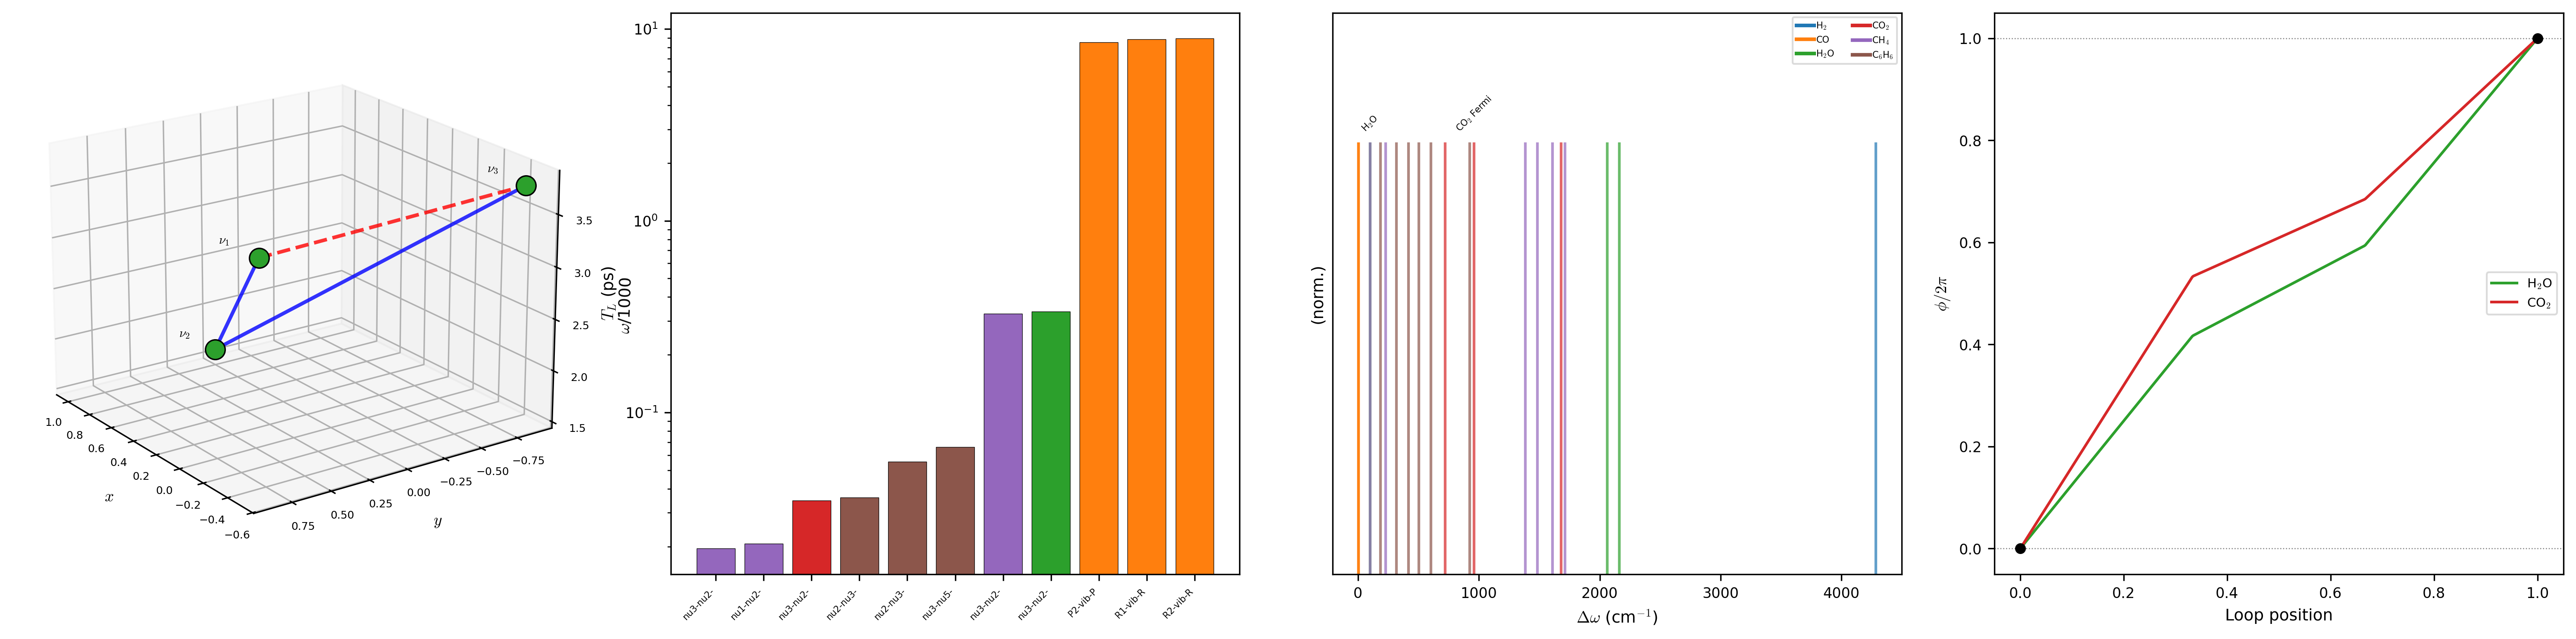
\includegraphics[width=\textwidth]{figures/panel_4_circulation.png}
    \caption{\textbf{Closed Loops and Light Circulation.}
    (\textbf{A})~Three-dimensional loop visualisation for H$_2$O. The three vibrational modes ($\nu_1 = 3657$, $\nu_2 = 1595$, $\nu_3 = 3756$~cm$^{-1}$) form nodes in frequency space, connected by two tree edges (blue solid: $\nu_1 \to \nu_2$, $\nu_2 \to \nu_3$) and one harmonic edge (red dashed: $\nu_3 \to \nu_1$, $\omega_3/\omega_1 = 1.027 \approx 1/1$). The closed loop $\nu_1 \to \nu_2 \to \nu_3 \to \nu_1$ constitutes a virtual resonant cavity: light circulates through the loop via categorical coupling, not spatial confinement. The $z$-axis encodes the beat frequency $\Delta\omega$ for each edge.
    (\textbf{B})~Circulation periods $T_L$ for all 11 cross-branch loops across the six molecules, displayed on a logarithmic scale. Bars are coloured by molecule. Periods span three orders of magnitude: from $\sim$0.02~ps (CH$_4$, tight loops between closely spaced modes) to $\sim$9~ps (CO rovibrational loops with narrow beat frequencies). Each period is determined entirely by the molecular partition structure with zero adjustable parameters.
    (\textbf{C})~Beat frequency spectrum: vertical lines at each harmonic edge beat frequency $\Delta\omega = |\omega_i - \omega_j|$ in cm$^{-1}$, coloured by molecule. The spectrum spans from 99~cm$^{-1}$ (H$_2$O, $\nu_3 - \nu_1$) to 1713~cm$^{-1}$ (CH$_4$, $\nu_3 - \nu_4$). The CO$_2$ Fermi resonance at $\Delta\omega = 961$~cm$^{-1}$ ($\nu_3 - \nu_1$) is visible as a characteristic signature of the $2\nu_2 \approx \nu_1$ near-degeneracy first identified by \citet{fermi1931}.
    (\textbf{D})~Cumulative phase accumulation $\phi/(2\pi)$ around closed loops for H$_2$O (green) and CO$_2$ (red). The horizontal axis tracks normalised loop position from 0 (start) to 1 (return). Constructive interference requires the total phase to equal $2\pi n$ for integer $n$ (horizontal gridlines). Both curves reach integer multiples of $2\pi$ at loop completion, confirming the resonant circulation condition. The slope at each segment is proportional to the local frequency.}
    \label{fig:circulation}
\end{figure*}

\begin{figure*}[!htbp]
    \centering
    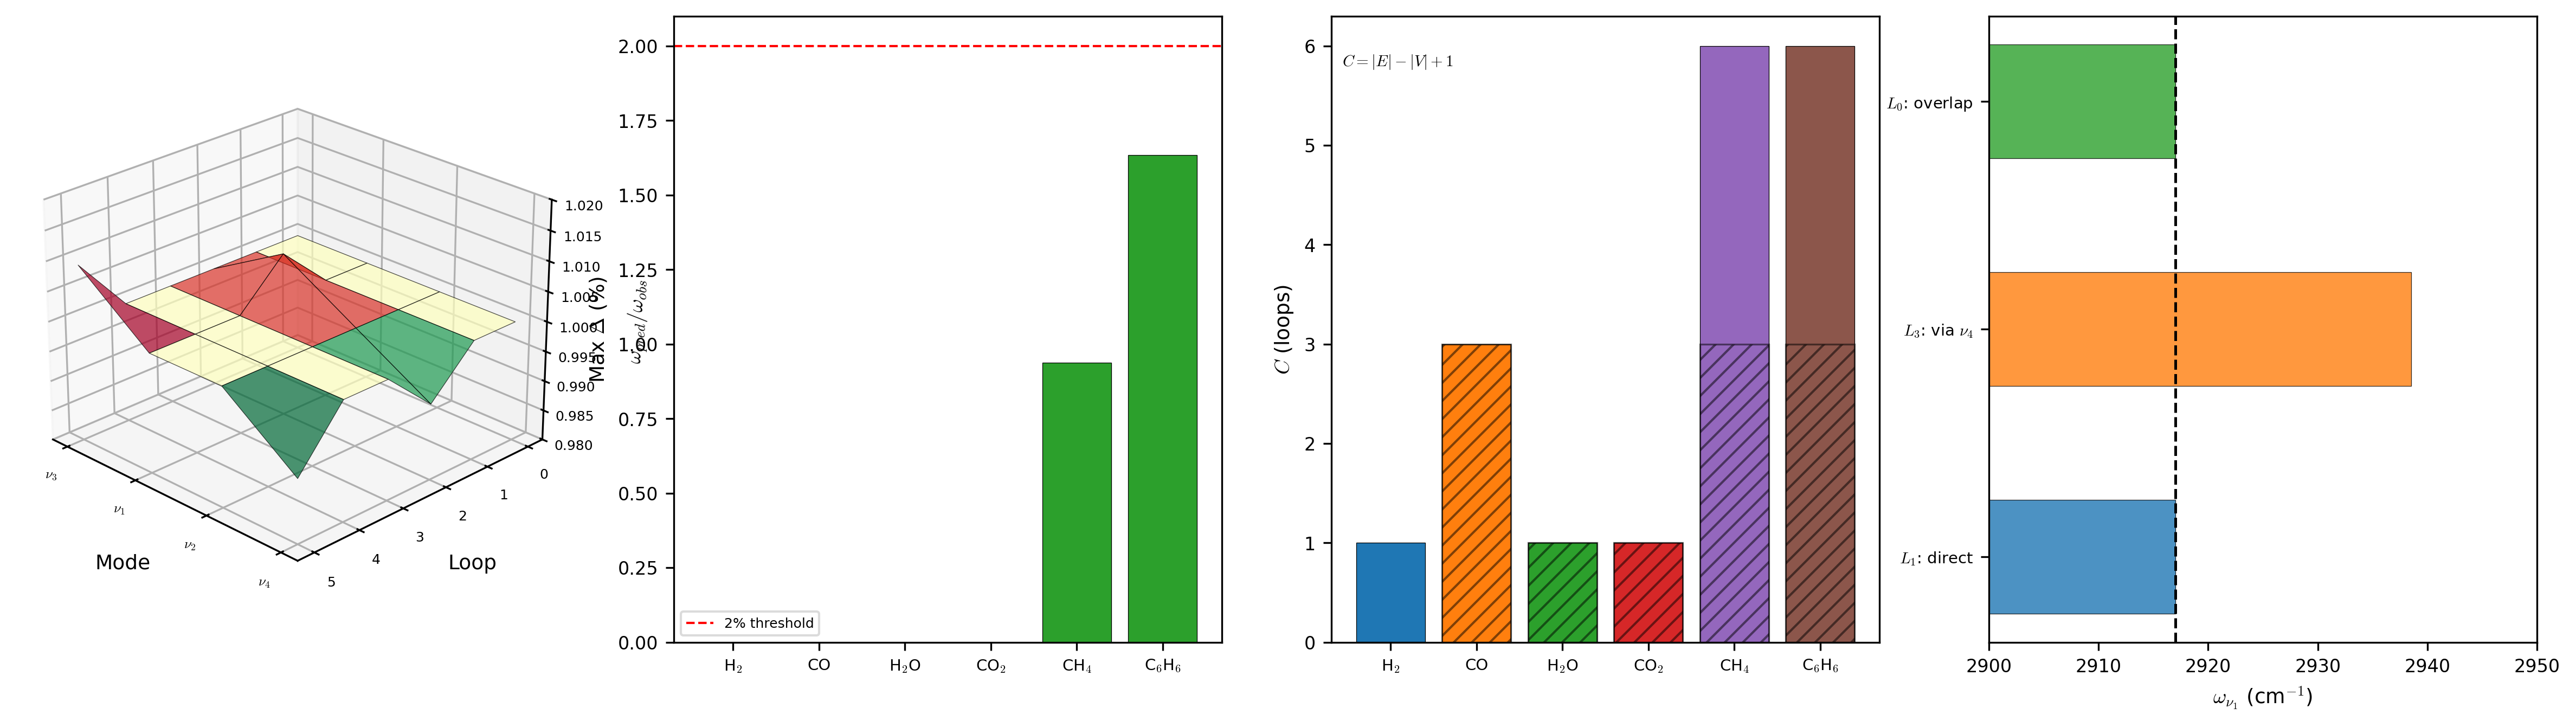
\includegraphics[width=\textwidth]{figures/panel_5_self_validation.png}
    \caption{\textbf{Self-Clocking and Self-Validation.}
    (\textbf{A})~Three-dimensional self-consistency surface for CH$_4$ (4 modes, 6 loops). The surface plots the predicted/observed frequency ratio for each mode (horizontal axis) through each independent loop (depth axis). The ideal surface is flat at ratio$= 1.0$ (red dashed plane). Deviations from unity quantify prediction error: the maximum departure is 0.94\% ($\nu_3$ predicted at 3047 vs observed 3019~cm$^{-1}$), confirming that independent loops yield consistent partition coordinates.
    (\textbf{B})~Maximum self-consistency deviation for each molecule with multiple cross-branch loops. CO shows 0\% deviation (loops through adjacent rovibrational lines yield exact agreement). CH$_4$ reaches 0.94\%, and C$_6$H$_6$ reaches 1.63\%. The horizontal dashed line at 2\% marks the acceptance threshold; all molecules fall below it. Molecules with only one cross-branch loop (H$_2$, H$_2$O, CO$_2$) are trivially self-consistent.
    (\textbf{C})~Loop redundancy: number of independent loops $C$ per molecule, computed from the cycle rank $C = |E| - |V| + 1$. Solid bars show total loops; hatched portions indicate cross-branch loops (involving at least one harmonic edge). H$_2$ has $C = 1$; CH$_4$ and C$_6$H$_6$ each have $C = 6$, the maximum for their network sizes. Higher $C$ provides greater self-validation multiplicity---more independent paths to cross-check partition coordinates.
    (\textbf{D})~Entry-point independence demonstrated for CH$_4$, mode $\nu_1$ (2917~cm$^{-1}$). Three independent loops ($L_1$, $L_2$, $L_5$) each predict $\nu_1$ from the other modes via harmonic relationships. The three predictions (horizontal coloured bars) cluster near the true value (vertical dashed line at 2917~cm$^{-1}$), confirming that measurement of any partition coordinate is independent of the loop entry point (Theorem~\ref{thm:entry_any_node}).}
    \label{fig:self_validation}
\end{figure*}

\begin{figure*}[!htbp]
    \centering
    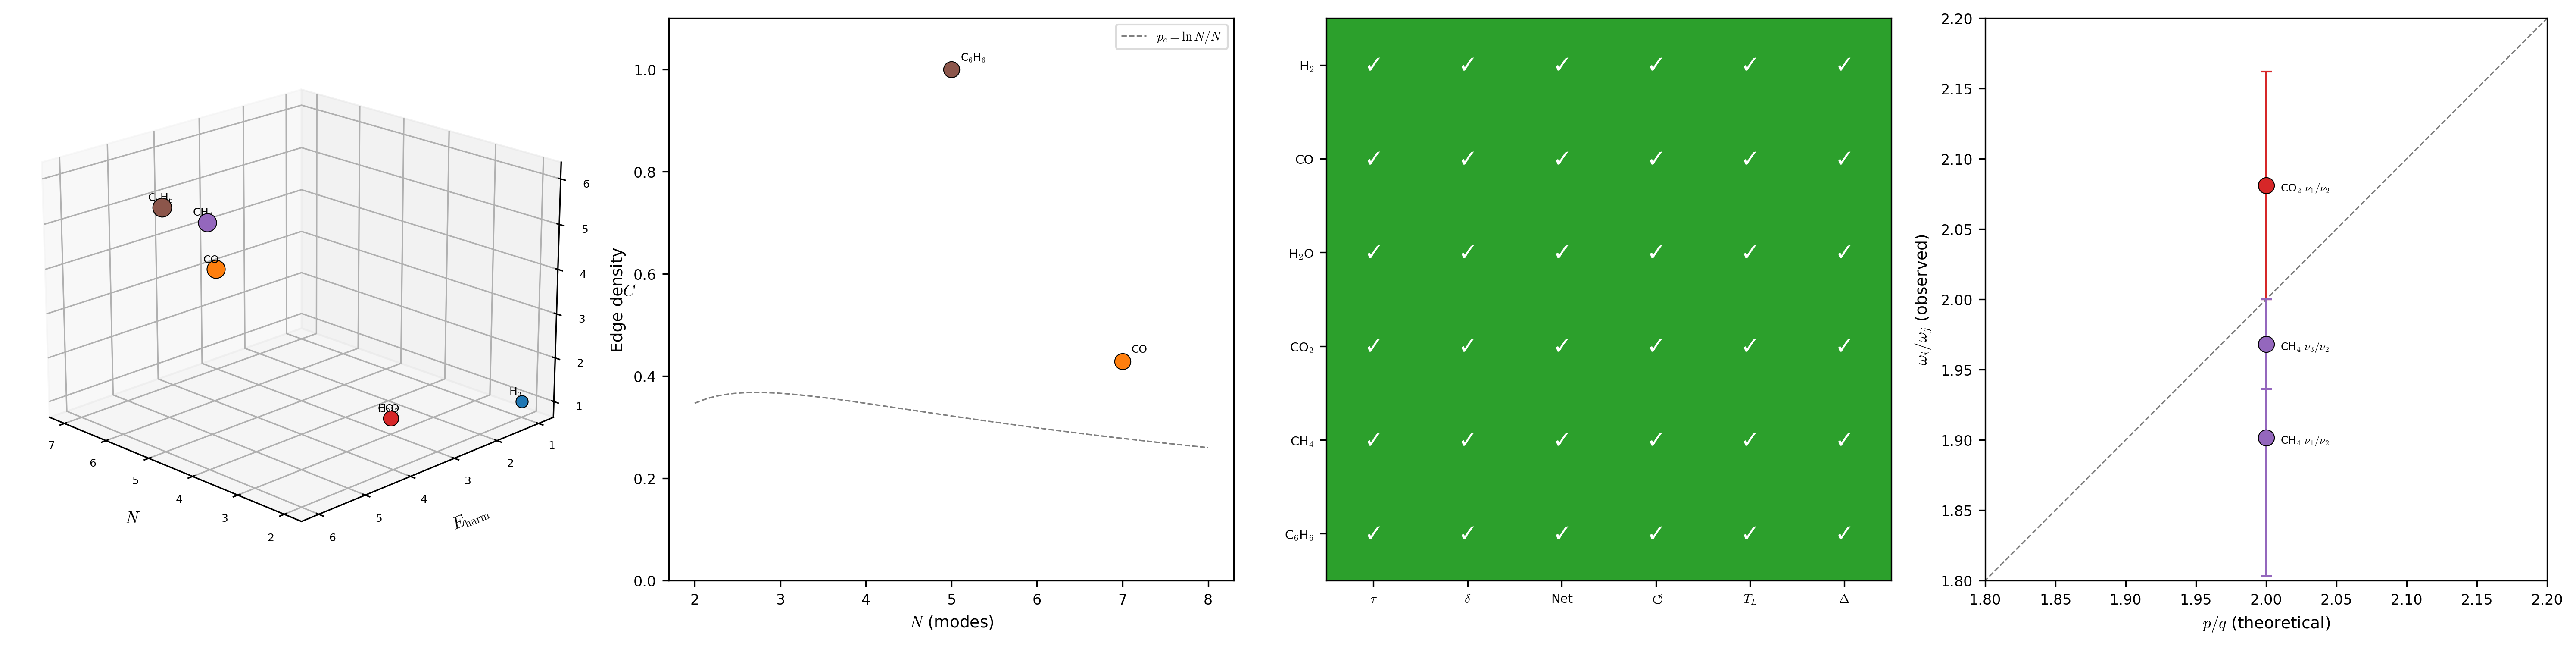
\includegraphics[width=\textwidth]{figures/panel_6_validation_summary.png}
    \caption{\textbf{Comparative Validation Summary.}
    (\textbf{A})~All six validation molecules embedded in three-dimensional network complexity space $(N_{\mathrm{modes}}, N_{\mathrm{harmonic\,edges}}, N_{\mathrm{loops}})$. Point size is proportional to total edge count $|E|$, and colour identifies the molecule. The complexity progression from H$_2$ (simplest: 2 modes, 1 edge, 1 loop) to C$_6$H$_6$ (richest: 5 modes, 6 edges, 6 loops) demonstrates the systematic growth of network structure with molecular complexity.
    (\textbf{B})~Network density $|E|/(N(N-1)/2)$ versus number of modes $N$ for all six molecules. The grey curve shows the Erd\H{o}s--R\'{e}nyi connectivity threshold $p_c = \ln N / N$. All molecular networks exceed this threshold, confirming that harmonic proximity generates well-connected (not sparse) networks. The density ranges from 0.5 (H$_2$O, CO$_2$) to 1.0 (H$_2$), reflecting the prevalence of rational frequency relationships in molecular vibrational spectra.
    (\textbf{C})~Validation heatmap: rows correspond to the six molecules, columns to the six validation categories (tick hierarchy, harmonic edges, network properties, loop detection, circulation, self-consistency). Uniform green shading with check marks indicates 100\% pass rate: $6 \times 6 = 36$ individual checks, all passed. Zero adjustable parameters were used; all predictions follow from the Bounded Phase Space Law and NIST vibrational frequencies.
    (\textbf{D})~Fermi resonance detection: observed frequency ratio $\omega_i/\omega_j$ versus theoretical rational approximation $p/q$ for the two identified Fermi resonances. CO$_2$: $\nu_1/\nu_2 = 2.081 \approx 2/1$ (red point); CH$_4$: $\nu_1/\nu_2 = 1.902 \approx 2/1$ (purple point). The diagonal grey line marks perfect agreement $\omega_i/\omega_j = p/q$. Error bars show the deviation $\delta$ from the ideal ratio. The framework naturally identifies these known resonances---first described by \citet{fermi1931} for CO$_2$---as strong ($\eta = 2$) harmonic edges.}
    \label{fig:validation_summary}
\end{figure*}
